\section{Motivations}
    
\subsection{Motivations générales}    
    \begin{frame}
        \frametitle{Exploration spatiale : les motivations}
        L'observation et l'acquisition de données scientifiques directement à la surface d'une planète permettent d'obtenir des informations riches :
        \begin{itemize}
            \item Comprendre l'univers et son origine \cite{motivation1} ;
            \item Découvrir des traces de vie extraterrestre \cite{motivation2} ;
            \item Acquérir des ressources naturelles \cite{motivation2} ;
            \item Coloniser de nouvelles planètes \cite{motivation1} ;
            \item etc.
        \end{itemize}
    \end{frame}
    
\subsection{Mise en contexte}
    \begin{frame}
        \begin{center}
        \begin{figure}
            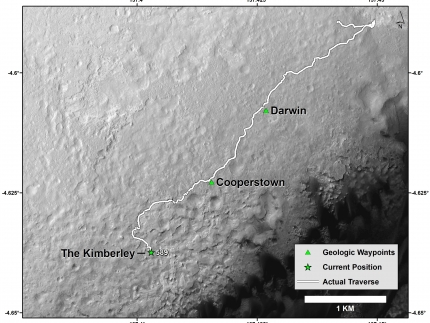
\includegraphics[height=0.4\textheight]{./media/landing.jpg}
            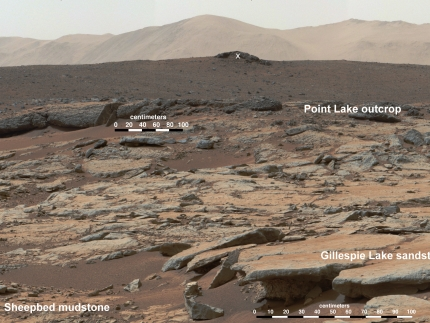
\includegraphics[height=0.4\textheight]{./media/geometry2.jpg}\\
            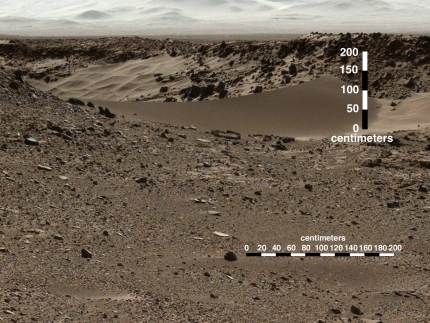
\includegraphics[height=0.4\textheight]{./media/geometry.jpg}
            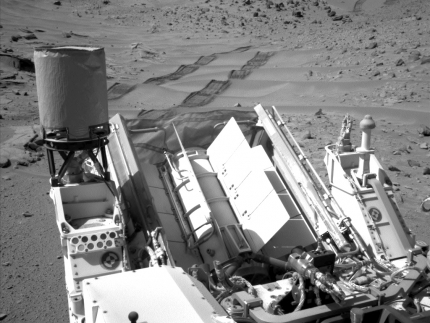
\includegraphics[height=0.4\textheight]{./media/wheelSand.jpg}
            \caption{Mars observé par le robot Curiosity \cite{nasa}}
        \end{figure}            
        \end{center} 
        \note{Zone où se poser = parcourir longue distance} 
        \note{Mécanique terrain vs robot}
        \note{Géométrie du terrain et interaction terrain-robot}
        \note{Immobilisation, délais, compromettre la mission}
        \note{Principale difficulté : identification autonome les zones naviagbles}
        \note{Téléopération 24h}        
    \end{frame}
    
    \begin{frame}
        \frametitle{Exemples d'échecs}
        L'une des principales difficultés de la navigation pour les robots est l'identification autonome des régions pouvant être traversées sécuritairement.   
        \begin{itemize}
            \item Opportunity 2005 : délais d'un mois pour dégager le véhicule \cite{Brooks2012} ;
            \item Spirit 2009 : immobilisation complète \citep{spirit} ;
            \item Opportunity 2010 : fin de la mission à cause de l'immobilisation \cite{Brooks2012}.
        \end{itemize}
    \end{frame}
    
\subsection{Objectif}
    \begin{frame}[c]
        \frametitle{Objectif de l'article}
        \textbf{Développer une technique permettant d'identifier de manière autonome les terrains potentiellement dangereux à distance, lorsque l'apparence visuelle du terrain n'est pas connue à priori.}
    \end{frame}